\chapter{Implementacija i korisničko sučelje}
		
		
		\section{Korištene tehnologije i alati}
		
			 Komunikacija među članovima projektnog tima ostvarena je pomoću platforme  \underline{Microsoft Teams} \footnote{https://www.microsoft.com/en-us/microsoft-365/microsoft-teams/group-chat-software} preko koje su održavani video sastanci te pomoću mobilne aplikacije za razmjenu poruka \underline{WhatsApp}  \footnote{https://www.whatsapp.com}. Za pisanje dokumentacije korišten je programski jezik za dokumente \underline{LaTeX} \footnote{https://www.latex-project.org/} i LaTeX uređivač \underline{Texstudio} \footnote{https://www.texstudio.org/}, za izradu različitih UML dijagrama korišten je alat \underline{Astah UML} \footnote{https://astah.net/products/astah-community/}, dok je za izradu ER dijagrama baze podataka korišten alat za baze podataka \underline{DBeaver} \footnote{https://dbeaver.io/}. Za upravljanje inačicama datoteka projekta korišten je distribuirani sustav \underline{Git} \footnote{https://git-scm.com/}, a repozitorij projektne grupe uspostavljen je na \underline{GitLabu} \footnote{https://about.gitlab.com/}. GitLab je web hosting usluga koja podržava rad sustava Git.
			 
			 Za razvojno okruženje korišten je \underline{IntelliJ IDEA} \footnote{https://www.jetbrains.com/idea/}, integrirano razvojno okruženje (IDE) koje je razvila tvrtka JetBrains. Ponajviše je namijenjeno za Javu, no podržava i mnogo drugih programskih jezika kao što su Kotlin, Scala, Python i drugi. Koristi se za razvoj, modeliranje i \textit{deployment} web i mobilnih aplikacija. 
			 
			 Za izradu web aplikacije korišten je radni okvir \underline{Spring Boot} \footnote{https://spring.io/projects/spring-boot} uz arhitekturni stil \underline{Rest API} \footnote{https://restfulapi.net/} koji se bazira na HTTP protokolu. Spring Boot je specijalizacija radnog okvira Spring a omogućuje jednostavnije i brže oblikovanje web aplikacija tako što u svojoj automatskoj konfiguraciji neke uobičajene dijelove web aplikacije već ima podešeno, kao na primjer pokretanje Apache Tomcat poslužitelja. Od programskih jezika koriste se objektno orijentirani jezik \underline{Java} \footnote{https://www.java.com/en/} za izradu \textit{backend} sloja aplikacije te skriptni programski jezik \underline{JavaScript} \footnote{https://www.javascript.com/} te knjižnica \underline{React} \footnote{https://reactjs.org/}  za izradu \textit{frontend} sloja. Uz Javu smo koristili \underline{Apache Maven} \footnote{https://maven.apache.org/}, \textit{open source} alat za tehničko upravljanje Java projektima. Knjižnicu React razvija tvrtka Facebook a pisana je u jeziku JavaScript i sadrži mnogo paketa te je tako fleksibilna za različite aplikacije. 
			 
			 Za rad s bazom podataka korišten je sustav za upravljanje bazom podataka \underline{PostgreSQL} \footnote{https://www.postgresql.org/} te alat za mapiranje podataka između relacijske baze i objekata u Javi \underline{Hibernate ORM} \footnote{https://hibernate.org/orm/}. Hibernate implementira standard Java Persistance API te nudi anotacije koje služe za lakši rad s entitetima.
			 
			 Baza podataka nalazi se na poslužitelju \underline{Heroku} \footnote{https://www.heroku.com/}
			
			
			\eject 
		
	
		\section{Ispitivanje programskog rješenja}
			
			\textbf{\textit{dio 2. revizije}}\\
			
			 \textit{U ovom poglavlju je potrebno opisati provedbu ispitivanja implementiranih funkcionalnosti na razini komponenti i na razini cijelog sustava s prikazom odabranih ispitnih slučajeva. Studenti trebaju ispitati temeljnu funkcionalnost i rubne uvjete.}
	
			
			\subsection{Ispitivanje komponenti}
			\textit{Potrebno je provesti ispitivanje jedinica (engl. unit testing) nad razredima koji implementiraju temeljne funkcionalnosti. Razraditi \textbf{minimalno 6 ispitnih slučajeva} u kojima će se ispitati redovni slučajevi, rubni uvjeti te izazivanje pogreške (engl. exception throwing). Poželjno je stvoriti i ispitni slučaj koji koristi funkcionalnosti koje nisu implementirane. Potrebno je priložiti izvorni kôd svih ispitnih slučajeva te prikaz rezultata izvođenja ispita u razvojnom okruženju (prolaz/pad ispita). }
			
			
			
			\subsection{Ispitivanje sustava}
			
		 	
		 	\noindent \underbar{\textbf{Ispitni slučaj: UC2 - Registracija, osnovni tijek}}
		 	\begin{packed_item}
		 		
		 	\item  \textbf{Ulaz:}
		 		
		 		\item[] \begin{packed_enum}
		 			
		 			\item Korisnik otvara stranicu za registraciju
		 			\item Korisnik unosi svoje podatke
		 			\item Korisnik pritišće tipku "Registriraj se"
		 			
		 		\end{packed_enum}
	 		
	 		\item \textbf{Očekivani rezultat:}
	 			
	 				\item[] \begin{packed_enum}
	 				
	 				\item Korisnik se uspješno registrirao
	 				\item Korisnik je preusmjeren na početnu stranicu
	 				
	 			\end{packed_enum}		
 			
 			\item \textbf{Rezultat:} 
 			
 					\item[] \begin{packed_enum}
 						
 						\item Korisnik je registriran i preusmjeren na početnu stranicu
 						
 					\end{packed_enum}	
 				
 							
		 		
		 	\end{packed_item}
	 	
	 		\begin{figure}[H]		
	 			\begin{figure}[H]
	 				\begin{subfigure}{0.5\textwidth}
	 					\centering
	 					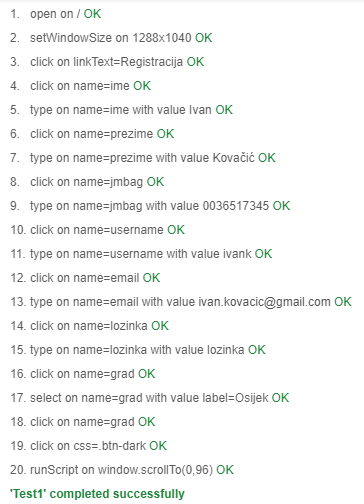
\includegraphics[scale=0.7]{slike/test1.png}
	 					\caption{Prvi ispitni slučaj: provedeni test}
	 					\label{fig:prviIspitniSlucajTest}
	 				\end{subfigure}%			
	 			\end{figure}
	 		\end{figure}
	 	
	 		
 		
 			\noindent \underbar{\textbf{Ispitni slučaj: UC2 - Registracija, odstupanje}}
 			\begin{packed_item}
 				
 				\item  \textbf{Ulaz:}
 				
 				\item[] \begin{packed_enum}
 					
 					\item Korisnik otvara stranicu za registraciju
 					\item Korisnik unosi podatke i izabire korisničko ime koje već postoji
 					\item Korisnik pritišće tipku "Registriraj se"
 					
 				\end{packed_enum}
 				
 				\item \textbf{Očekivani rezultat:}
 				
 				\item[] \begin{packed_enum}
 					
 					\item Sustav vraća korisnika na stranicu za registraciju s upisanim podacima i porukom o pogrešci
 					
 				\end{packed_enum}		
 				
 				\item \textbf{Rezultat:} 
 				
 				\item[] \begin{packed_enum}
 					
 					\item Registracija nije uspješna i korisnik je vraćen na stranicu za registraciju s upisanim podacima i porukom o pogrešci
 					
 				\end{packed_enum}
 					
 				
 			\end{packed_item}
 		
 		
 			\begin{figure}[H]
 				\centering
 				\begin{subfigure}{.5\textwidth}
 					\centering
 					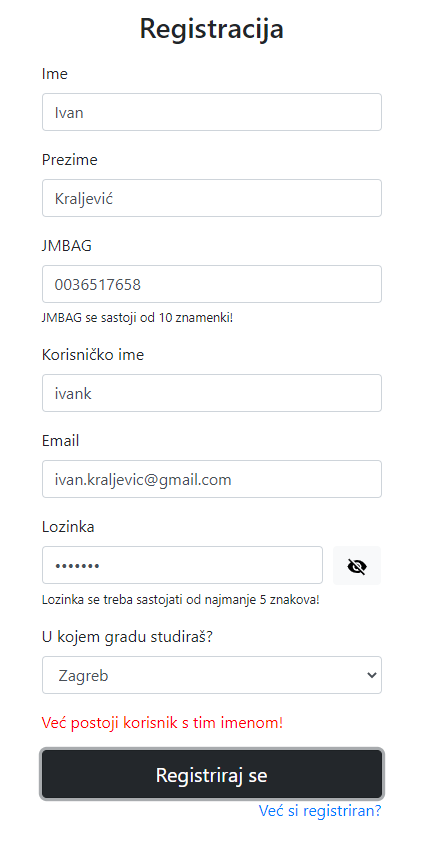
\includegraphics[scale=0.3]{slike/test2Ekran.png}
 					\caption{Drugi ispitni slučaj: rezultat}
 					\label{fig:drugiIspitniSlucaj}
 				\end{subfigure}%
 				\begin{subfigure}{.5\textwidth}
 					\centering
 					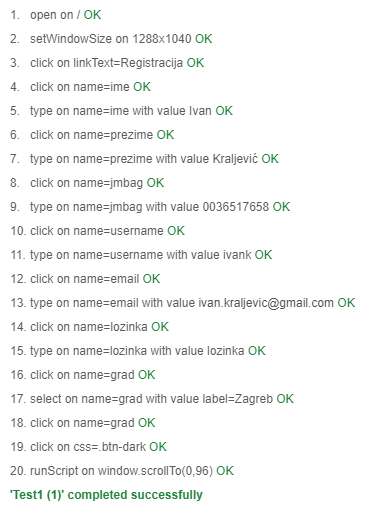
\includegraphics[scale=0.5]{slike/test2.png}
 					\caption{Drugi ispitni slučaj: provedeni test}
 					\label{fig:drugiIspitniSlucajTest}%
 				\end{subfigure}
 			\end{figure}
 			
 			\noindent \underbar{\textbf{Ispitni slučaj: UC3 - Prijava u sustav, osnovni tijek}}
 			\begin{packed_item}
 				
 				\item  \textbf{Ulaz:}
 				
 				\item[] \begin{packed_enum}
 					
 					\item Korisnik otvara stranicu za prijavu
 					\item Korisnik unosi svoje podatke
 					\item Korisnik pritišće tipku "Prijavi se"
 					
 				\end{packed_enum}
 				
 				\item \textbf{Očekivani rezultat:}
 				
 				\item[] \begin{packed_enum}
 					
 					\item Korisnik se uspješno prijavio
 					\item Korisnik je preusmjeren na početnu stranicu
 					
 				\end{packed_enum}		
 				
 				\item \textbf{Rezultat:} 
 				
 					\begin{packed_enum}
 						
 						\item Korisnik je prijavljen i preusmjeren na početnu stranicu
 						
 					\end{packed_enum}
 						
 				
 			\end{packed_item}
 			
 			\begin{figure}[H]
 				\begin{subfigure}{0.5\textwidth}
 					\centering
 					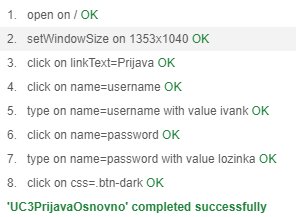
\includegraphics[scale=0.7]{slike/test3.png}
 					\caption{Treći ispitni slučaj: provedeni test}
 					\label{fig:treciIspitniSlucajTest}
 				\end{subfigure}%
 			
 			\end{figure}
 		
 		\noindent \underbar{\textbf{Ispitni slučaj: UC3 - Prijava u sustav, odstupanje}}
 		\begin{packed_item}
 			
 			\item  \textbf{Ulaz:}
 			
 			\item[] \begin{packed_enum}
 				
 				\item Korisnik otvara stranicu za prijavu
 				\item Korisnik unosi korisničko ime koje ne postoji
 				\item Korisnik pritišće tipku "Prijavi se"
 				
 			\end{packed_enum}
 			
 			\item \textbf{Očekivani rezultat:}
 			
 			\item[] \begin{packed_enum}
 				
 				\item Sustav javlja poruku o pogrešci
 				\item Prijava nije uspješna
 				
 			\end{packed_enum}		
 			
 			\item \textbf{Rezultat:} 
 			
 			\begin{packed_enum}
 				
 				\item Sustav javlja poruku o nepostojanju korisničkog imena
 				\item Prijava nije uspješna
 				
 			\end{packed_enum}
 			
 			
 		\end{packed_item}
 	
 	
 		
 			\begin{figure}[H]
 			\centering
 			\begin{subfigure}{.5\textwidth}
 				\centering
 				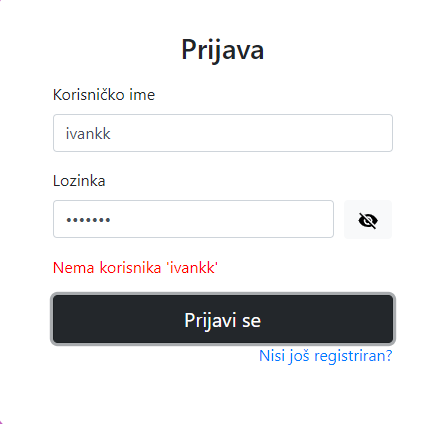
\includegraphics[scale=0.4]{slike/test4Ekran.png}
 				\caption{Četvrti ispitni slučaj: rezultat}
 				\label{fig:cetvrtiIspitniSlucaj}
 			\end{subfigure}%
 			\begin{subfigure}{.5\textwidth}
 				\centering
 				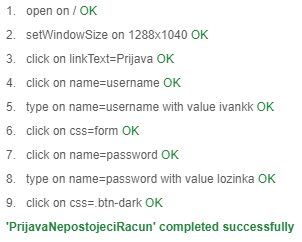
\includegraphics[scale=0.7]{slike/test4.png}
 				\caption{Četvrti ispitni slučaj: provedeni test}
 				\label{fig:cetvrtiIspitniSlucajTest}%
 			\end{subfigure}
 		\end{figure}
 	
 		\noindent \underbar{\textbf{Ispitni slučaj: UC13 - Promjena profila, osnovni tijek}}
 		\begin{packed_item}
 			
 			\item  \textbf{Ulaz:}
 			
 			\item[] \begin{packed_enum}
 				
 				\item Korisnik otvara stranicu profila
 				\item Korisnik pritišće tipku 'Uredi'
 				\item Korisnik mijenja svoje podatke
 				\item Korisnik pritišće tipku "Ažuriraj podatke"
 				
 			\end{packed_enum}
 			
 			\item \textbf{Očekivani rezultat:}
 			
 			\item[] \begin{packed_enum}
 				
 				\item Ažurirani podaci vidljivi su na stranici profila
 				
 			\end{packed_enum}		
 			
 			\item \textbf{Rezultat:} 
 			
 			\begin{packed_enum}
 				
 				\item Ažurirani podaci vidljivi su na stranici profila
 				
 			\end{packed_enum}
 			
 			
 		\end{packed_item}
 	
 	\begin{figure}[H]
 		\centering
 		\begin{subfigure}{.5\textwidth}
 			\centering
 			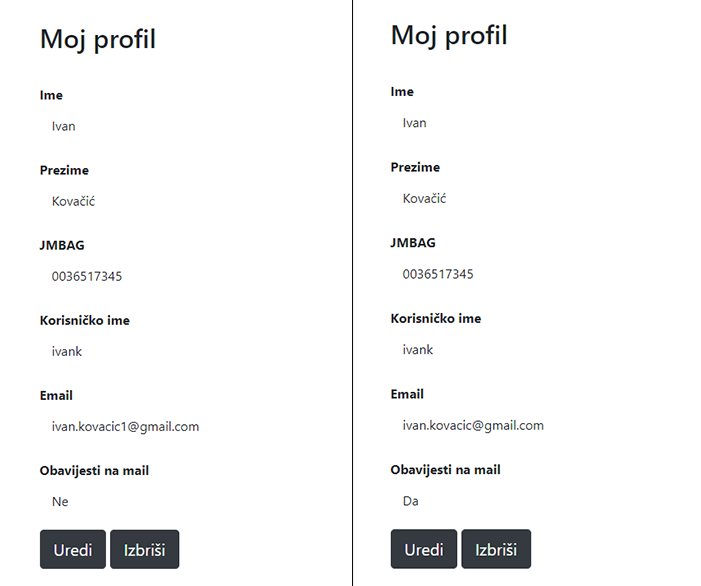
\includegraphics[scale=1.5]{slike/test5Ekran.png}
 			\caption{Peti ispitni slučaj: rezultat}
 			\label{fig:petiIspitniSlucaj}
 		\end{subfigure}%
 		\begin{subfigure}{.5\textwidth}
 			\centering
 			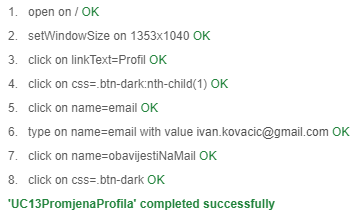
\includegraphics[scale=0.7]{slike/test5.png}
 			\caption{Peti ispitni slučaj: provedeni test}
 			\label{fig:petiIspitniSlucajTest}%
 		\end{subfigure}
 	\end{figure}
 		
 		
 		
 		\eject 
			
			\eject 
		
		
		\section{Dijagram razmještaja}
		
			Dijagram razmještaja statički je UML dijagram koji prikazuje i opisuje topologiju sustava te programsku potporu za implementaciju sustava. Korisnik, to jest klijent na svom osobnom računalu koristi web preglednik za pristup web aplikaciji. Na poslužiteljskom računalu nalazi se Tomcat web poslužitelj te PostgreSQL poslužitelj baze podataka. Komunikacija između klijenta i poslužitelja odvija se preko protokola aplikacijskog sloja HTTP.
			
			\begin{figure}[H]
				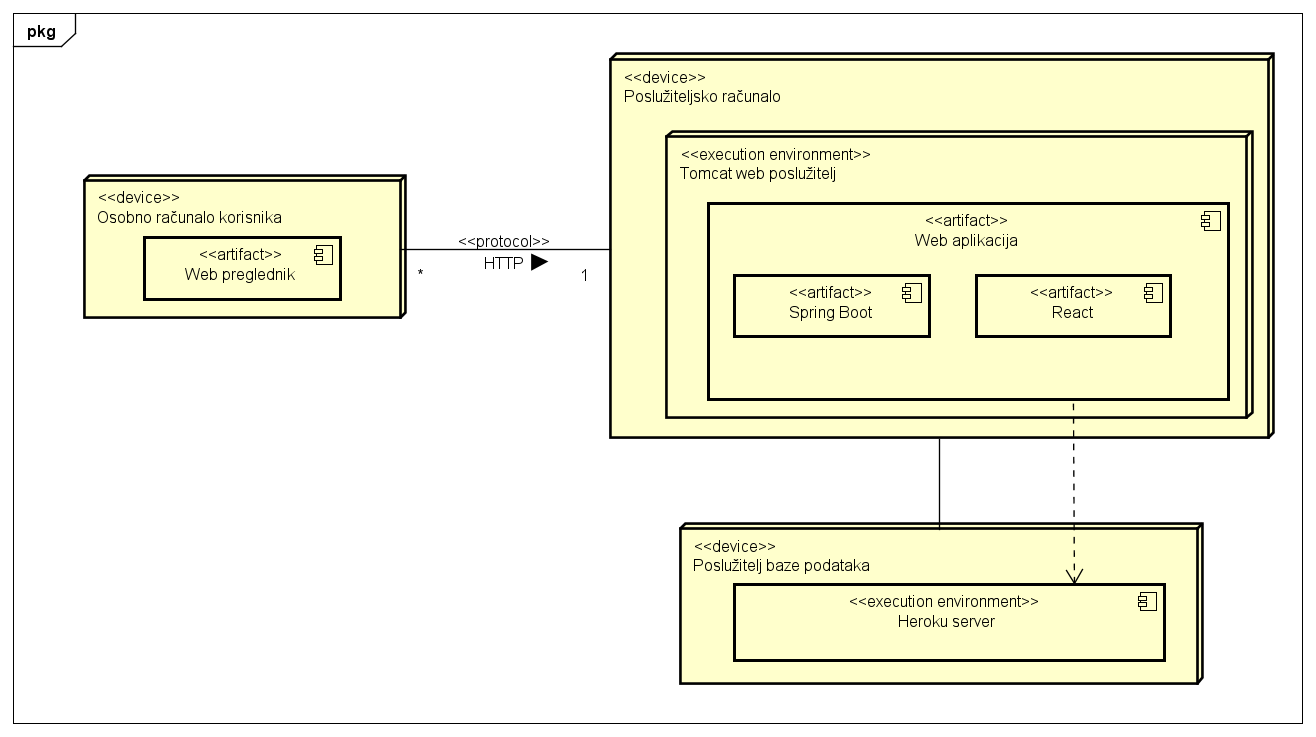
\includegraphics[scale=0.4]{dijagrami/dijagramRazmjestaja1} %veličina slike u odnosu na originalnu datoteku i pozicija slike
				\centering
				\caption{Dijagram razmještaja}
				\label{fig:dijagramRazmjestaja}
			\end{figure}
			
			 
			\eject 
		
		\section{Upute za puštanje u pogon}
		
		
			\textbf{Git}
			\\Ako sustav Git nije instaliran, potrebno je preuzeti instalacijski paket s poveznice \href{https://git-scm.com/downloads}{https://git-scm.com/downloads}.
			\begin{packed_item}
				\item Instalacija
				\begin{packed_enum}
					\item Pokrenuti preuzeti instalacijski program čime se otvara čarobnjak za konfiguraciju
					\item Odabrati direktorij za instalaciju
					\item Ostaviti zadane izabrane komponente
					\item Za path varijablu odabrati \textit{Git from the command line and also from 3-rd party software}
					\item Odabrati \textit{Use the OpenSSL library}
					\item Odabrati \textit{Checkout windows-style, commit Unix-style line endings } (za operacijski sustav Windows)
					\item Odabrati \textit{Use Windows' default console window}
					\item Odabrati \textit{Default (fast-forward or merge)}
					\item Ostaviti zadane dodatne postavke
					\item Pritisnuti \textit{Install}
				\end{packed_enum}
				\item Konfiguracija
				\\Detalji konfiguracije mogu se proučiti na stranici \href{https://git-scm.com/book/en/v2/Getting-Started-First-Time-Git-Setup}{First-Time Git Setup}
			\end{packed_item}
			\
			\textbf{Apache Maven}
			\\Ako alat Apache Maven nije instaliran, potrebno je preuzeti instalacijski paket s poveznice 	\href{https://maven.apache.org/download.cgi}{https://maven.apache.org/download.cgi}
				\begin{packed_enum}
					\item Preuzeti \textit{Binary zip archive}
					\item Raspakirati distribuciju arhive u željeni direktorij
					\item U Windows Start upisati i odabrati \textit{Uređivanje varijabli okruženja sustava} (\textit{Edit the system environment variables}) 
					\item Odabrati \textit{Varijable okruženja} (\textit{Environment variables})
					\item U PATH sistemsku varijablu dodati bin direktorij stvorenog apache-maven direktorija
					\item U naredbenom retku naredbom \texttt{mvn -v} provjeriti uspješnost instalacije
				\end{packed_enum}
			\begin{figure}[H]
				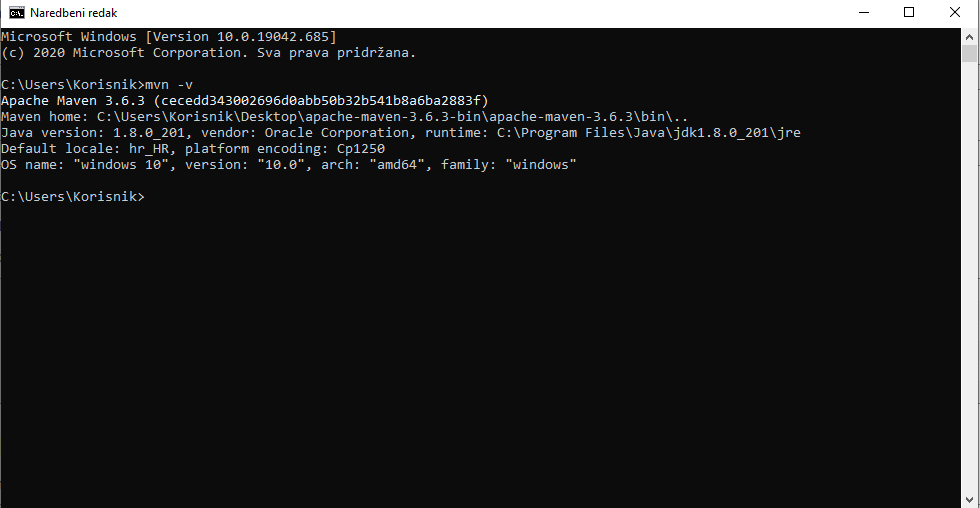
\includegraphics[scale=0.5]{slike/maven} %veličina slike u odnosu na originalnu datoteku i pozicija slike
				\centering
				\caption{Ispravna instalacija}
				\label{fig:mavenIspravnaInstalacija}
			\end{figure}
			\
			\textbf{Heroku klijent}
			\\Na stranici \href{https://www.heroku.com/}{https://www.heroku.com/} potrebno je napraviti korisnički račun. Nakon toga treba preuzeti instalacijski paket s poveznice \url{https://devcenter.heroku.com/articles/heroku-cli}.
				\begin{packed_enum}
					\item Pokrenuti preuzeti instalacijski program čime se otvara čarobnjak za konfiguraciju
					\item Ostaviti zadane komponente
					\item Odabrati direktorij za instalaciju
					\item U naredbenom retku naredbom \texttt{heroku version} provjeriti uspješnost instalacije
				\end{packed_enum}
			\
			\textbf{Postupak puštanja u pogon}
				\begin{packed_item}
					\item Stvaranje Heroku servera za backend dio
					\begin{packed_enum}
						\item U naredbenom retku upisati \texttt{heroku login} i ulogirati se
						\item Upisati \texttt{heroku create <NAME-OF-APP>}
					\end{packed_enum}
				\end{packed_item}
			
				\begin{packed_item}
					\item Stvaranje baze
					\begin{packed_enum}
						\item Otvoriti stranicu \href{https://www.heroku.com/}{https://www.heroku.com/} 
						\item Kliknuti na NAME-OF-APP server
						\item Kliknuti na \textit{Resources}
						\item Odabrati \textit{Find more add-ons}
						\item Pronaći i odabrati \textit{Heroku POSTGRES}, odabrati plan \textit{Hobby Dev - Free}
					\end{packed_enum}
				\end{packed_item}
			
				\begin{packed_item}
					\item Konfiguracija backenda
					\begin{packed_enum}
						\item Kliknuti na NAME-OF-APP server
						\item Kliknuti na \textit{Resources}
						\item Kliknuti na \textit{Heroku POSTGRES}
						\item Kliknuti na \textit{Settings} i \textit{View Credentials}
						\item U projektnom direktoriju otvoriti \texttt{src/main/resources/application.properties}
						\item U datotetci podesiti podatke s View Credentials:
							\begin{packed_item}
								\item \texttt{spring.datasource.url=jdbc:postgresql://<Host>}
								\item \texttt{spring.datasource.username=<User>}
								\item \texttt{spring.datasource.password=<Password>}
							\end{packed_item}
					\end{packed_enum}
				\end{packed_item}
			
					\begin{packed_item}
					\item Puštanje backenda u pogon
					\begin{packed_enum}
						\item U projektnom direktoriju otvoriti datotetku \texttt{pom.xml}
						\item U datoteku dodati \textit{Maven Plugin Configuration}
							\begin{verbatim}
							<plugin>
								<groupId>com.heroku.sdk</groupId>
								<artifactId>heroku-maven-plugin</artifactId>
								<version>3.0.3</version>
								<configuration>
								   <appName><NAME-OF-APP>-backend</appName>
								   <includeTarget>false</includeTarget>
								   <includes>
								     <include>target/${project.build.finalName}.jar</include>
								   </includes>
								<jdkVersion>${java.version}</jdkVersion>
								<processTypes>
								   <web>java $JAVA_OPTS -jar target/${project.build.finalName}.jar</web>
								</processTypes>
								</configuration>
							</plugin>
							\end{verbatim}
						\item U naredbenom retku pozicionirati se u \textit{root} backenda projekta
						\item U naredbeni redak upisati \texttt{mvn clean heroku:deploy}
					\end{packed_enum}
				\end{packed_item}
			
					\begin{packed_item}
					\item Stvaranje Heroku servera za frontend dio
					\begin{packed_enum}
						\item U naredbenom retku upisati \texttt{heroku login} i ulogirati se
						\item Upisati \texttt{heroku create <NAME-OF-FRONTEND-APP> --buildpack \url{https://github.com/mars/create-react-app-buildpack.git}}
						\item Stvoriti prazan direktorij
						\item U naredbenom retku pozicionirati se u stvoreni direktorij i ipisati \texttt{git init}
						\item U naredbenom retku upisati \texttt{heroku git:remote -a <NAME-OF-FRONTEND-APP>}
						\item U direktorij kopirati \textit{root} frontenda projekta
						\item U naredbenom retku upisati \texttt{git add.}
						\item U naredbenom retku upisati \texttt{git commit -m "Initital commit"}
						\item U naredbenom retku upisati \texttt{git push heroku master}
					\end{packed_enum}
					\begin{packed_item}
						\item Napomena: Za puštanje u pogon frontend dijela u \textit{rootu} front direktorija projekta treba se nalaziti datotetka \textit{static.json} u kojoj treba biti: \begin{verbatim}
							{
							   "root": "build/",
							   "clean_urls": false,
							   "routes": {
							      "/**": "index.html"
							   }
							}
						\end{verbatim}
					\end{packed_item}
				\end{packed_item}
			\eject 
